\documentclass[conference]{IEEEtran}
\IEEEoverridecommandlockouts

\usepackage{cite}
\usepackage{amsmath,amssymb,amsfonts}
\usepackage{graphicx}
\usepackage{textcomp}
\usepackage{xcolor}
\usepackage{booktabs}
\usepackage{array}
\usepackage{enumitem}
\usepackage{url}
\usepackage{tikz}
\usetikzlibrary{arrows.meta,positioning,fit}

\title{Evidence-Based Draft: A Post-Quantum Secure Tunnel for MAVLink Telemetry with Runtime AEAD and Scheduler Integration}

\author{\IEEEauthorblockN{First Author}
\IEEEauthorblockA{\textit{Affiliation}\\
City, Country\\
email@domain.com}
\and
\IEEEauthorblockN{Second Author}
\IEEEauthorblockA{\textit{Affiliation}\\
City, Country\\
email@domain.com}}

\begin{document}
\maketitle

\begin{abstract}
This draft reconstructs the architecture, implementation, and measured behavior of the secure-tunnel repository from verified code, benchmark artifacts, and protocol documentation only. The system implements a post-quantum secure tunnel for UAV telemetry in which a PQC handshake establishes transport keys, an AEAD-protected UDP data plane carries MAVLink traffic, and a scheduler layer evaluates controlled runtime transitions without changing frozen protocol semantics. The draft explains the protocol and implementation with direct file and function references, summarizes the benchmark methodology used in primitive, localhost, and MAVLink end-to-end campaigns, and records the main measured results, including a single confirmed post-rekey anomaly affecting the \texttt{aesgcm128} MAVLink run. The protocol baseline is frozen at \texttt{PROTOCOL\_VERSION = 1.0} and all findings in this draft are tied to that baseline.
\end{abstract}

\section{System Motivation and UAV Telemetry Context}
Unmanned aerial vehicle telemetry links carry command, state, and health information that must remain available and authenticated under constrained compute budgets. In this repository the target application is MAVLink telemetry transported through a secure tunnel that preserves a fixed protocol core while permitting scheduler-layer experimentation. The protocol baseline is explicitly frozen in \texttt{context/secure\_tunnel\_protocol\_spec.md} and \texttt{reports/CORE\_FREEZE\_EXPERIMENTAL\_BASELINE\_20260316.md}. Those documents define the invariants that may not change during experiments: handshake message sequence, AEAD packet format, nonce construction, replay window behavior, rekey lifecycle, control-plane semantics, and suite registry structure.

The code and artifacts indicate a design goal that is more specific than generic link encryption. The tunnel is intended to secure bidirectional MAVLink transport between a drone-side companion computer and a GCS-side operator stack while keeping end-to-end telemetry continuity measurable. The central engineering question throughout the repository is not only whether PQC primitives function correctly, but whether they can be integrated into a real telemetry path with acceptable round-trip latency, bounded rekey disruption, and controllable runtime adaptation.

\section{System Architecture}
\subsection{High-Level Roles and Channels}
The authoritative protocol description identifies two roles: the drone acts as the client for the TCP handshake and the GCS acts as the server. This is visible in the implementation and the extracted protocol specification. The data plane is encrypted UDP, while the handshake and a separate control plane use TCP. In code, transport setup is concentrated in \texttt{core/async\_proxy.py}; the control server is implemented in \texttt{core/control\_tcp.py}; and the protocol state machine for rekey coordination is implemented in \texttt{core/policy\_engine.py}.

The repository therefore implements three interacting planes:
\begin{enumerate}[leftmargin=*]
\item A handshake plane that performs PQC key establishment and confirmation.
\item A data plane that protects MAVLink datagrams with AEAD framing and replay protection.
\item A control plane that coordinates rekeys and scheduler-triggered transitions.
\end{enumerate}

\begin{figure}[htbp]
\centering
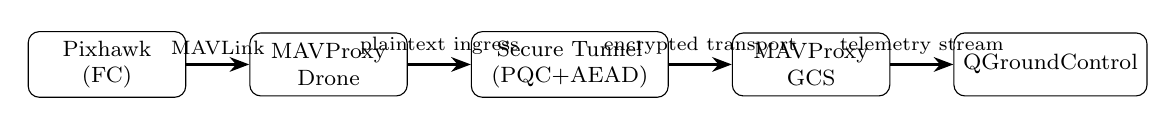
\begin{tikzpicture}[
node distance=0.8cm and 0.8cm,
box/.style={draw, rounded corners, minimum height=8mm, minimum width=20mm, align=center, font=\footnotesize},
arr/.style={-{Stealth[length=2.5mm]}, thick}
]
\node[box] (px) {Pixhawk\\(FC)};
\node[box, right=of px] (mpd) {MAVProxy\\Drone};
\node[box, right=of mpd, minimum width=25mm] (tun) {Secure Tunnel\\(PQC+AEAD)};
\node[box, right=of tun] (mpg) {MAVProxy\\GCS};
\node[box, right=of mpg] (qgc) {QGroundControl};

\draw[arr] (px) -- node[above, font=\scriptsize]{MAVLink} (mpd);
\draw[arr] (mpd) -- node[above, font=\scriptsize]{plaintext ingress} (tun);
\draw[arr] (tun) -- node[above, font=\scriptsize]{encrypted transport} (mpg);
\draw[arr] (mpg) -- node[above, font=\scriptsize]{telemetry stream} (qgc);
\end{tikzpicture}
\caption{System architecture path used in experiments: Pixhawk to MAVProxy on drone, through the secure tunnel, to MAVProxy on GCS and then QGroundControl.}
\label{fig:system-architecture}
\end{figure}

The proxy pipeline reconstructed from \texttt{core/async\_proxy.py} is: MAVProxy plaintext ingress, AEAD encryption, UDP transmission, AEAD decryption, control/data demultiplexing, and plaintext egress back into MAVProxy. The pipeline is not a synthetic crypto microbenchmark; it includes socket handling, peer validation, buffer draining, and control-message interaction, all of which matter when interpreting measured RTT.

\subsection{Frozen Baseline and Experimental Governance}
The freeze record in \texttt{reports/CORE\_FREEZE\_EXPERIMENTAL\_BASELINE\_20260316.md} states that experiments must operate on the frozen core implementation. That decision is crucial for interpreting the benchmark series. Primitive benchmarking, localhost tunnel validation, hardware deployment measurements, and scheduler evaluation were all meant to occur without modifying the transport semantics. As a result, scheduler experiments are explicitly a layer above protocol behavior rather than a rewrite of it.

\section{Protocol Design and Handshake Mechanism}
\subsection{Handshake Structure}
The handshake is implemented in \texttt{core/handshake.py}. The principal entry points are \texttt{server\_gcs\_handshake()} and \texttt{client\_drone\_handshake()}, while message parsing and transcript construction are handled by helper functions such as \texttt{\_parse\_server\_hello\_wire()} and \texttt{\_build\_server\_transcript()}. The server hello encoding is implemented directly in the file and matches the extracted protocol spec: version, KEM name length and bytes, signature name length and bytes, a 16-byte session identifier, a 16-byte challenge, the server KEM public key length and bytes, and the signature length and bytes.

The server transcript binds version, a protocol label, session identifier, KEM name, signature name, KEM public key, and challenge. The client verifies that transcript signature and additionally checks that the negotiated KEM and signature names match the expected suite. Those checks are the repository's downgrade barrier and are part of the frozen behavior. Once encapsulation and decapsulation succeed, \texttt{derive\_transport\_material()} derives 128 bytes of output keying material, split into directional transport keys and two key-confirmation values.

\begin{figure}[htbp]
\centering
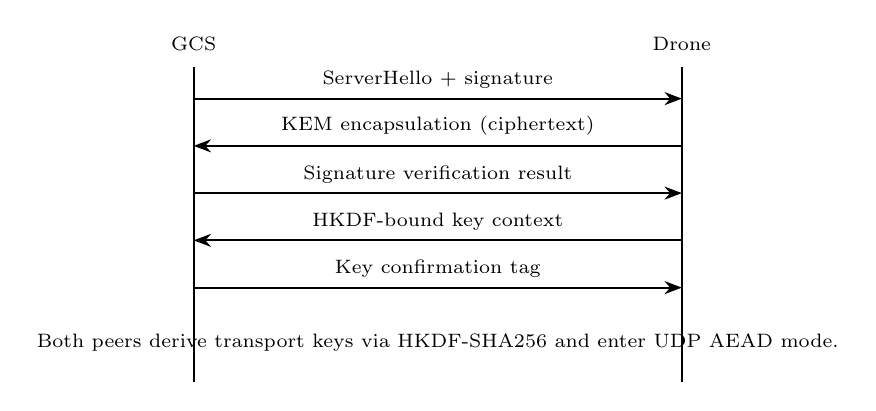
\begin{tikzpicture}[
x=1cm,y=1cm,
lifeline/.style={draw, thick},
msg/.style={-{Stealth[length=2.2mm]}, thick},
note/.style={font=\scriptsize, align=left}
]
\node[note] (gcs) at (0,4.3) {GCS};
\node[note] (drn) at (6.2,4.3) {Drone};
\draw[lifeline] (0,0) -- (0,4);
\draw[lifeline] (6.2,0) -- (6.2,4);

\draw[msg] (0,3.6) -- (6.2,3.6) node[midway, above, font=\scriptsize]{ServerHello + signature};
\draw[msg] (6.2,3.0) -- (0,3.0) node[midway, above, font=\scriptsize]{KEM encapsulation (ciphertext)};
\draw[msg] (0,2.4) -- (6.2,2.4) node[midway, above, font=\scriptsize]{Signature verification result};
\draw[msg] (6.2,1.8) -- (0,1.8) node[midway, above, font=\scriptsize]{HKDF-bound key context};
\draw[msg] (0,1.2) -- (6.2,1.2) node[midway, above, font=\scriptsize]{Key confirmation tag};

\node[note] at (3.1,0.5) {Both peers derive transport keys via HKDF-SHA256 and enter UDP AEAD mode.};
\end{tikzpicture}
\caption{Handshake lifecycle reflected by \texttt{core/handshake.py}: ServerHello, KEM encapsulation, verification, HKDF key derivation, and key confirmation.}
\label{fig:handshake-sequence}
\end{figure}

\subsection{Key Derivation and Confirmation}
The KDF in \texttt{derive\_transport\_material()} uses HKDF-SHA256 from the \texttt{cryptography} package. Its inputs are the KEM shared secret, the 16-byte session identifier, the 16-byte challenge, algorithm names, a PSK-derived digest, and the epoch value. The \texttt{info} field binds protocol and algorithm context, while the \texttt{salt} includes a PSK-derived component. The code therefore combines post-quantum shared secret material with pre-shared-key binding and explicit epoch context. Key confirmation uses HMAC-SHA256 over a transcript that includes the hello wire image and the KEM ciphertext. This is consistent with using HKDF as standardized in RFC~5869~\cite{rfc5869}.

\subsection{Suite Registry}
Suite metadata are managed in \texttt{core/suites.py}. The repository maintains a larger canonical registry, while the operational baseline highlighted in multiple reports repeatedly uses three runtime-allowed representative suites: \texttt{cs-mlkem512-mldsa44}, \texttt{cs-mlkem768-mldsa65}, and \texttt{cs-mlkem1024-mldsa87}. These correspond to NIST levels L1, L3, and L5 and are the pairings that appear in the measured localhost and MAVLink campaigns.

\section{AEAD Data Plane, Packet Framing, and Replay Protection}
\subsection{Wire Format}
The authenticated UDP framing is implemented in \texttt{core/aead.py}. The fixed header layout is defined by \texttt{HEADER\_STRUCT = !BBBBB\{SESSION\_ID\_LEN\}sQB}. That layout carries wire version, KEM identifier, KEM parameter, signature identifier, signature parameter, the 16-byte session identifier, a 64-bit sequence number, and a one-byte epoch. The sender constructs this header in \texttt{Sender.pack\_header()}, then uses it as AEAD associated data in \texttt{Sender.encrypt()}.

The on-wire format is header followed by ciphertext plus tag. The IV is not transmitted. This choice reduces packet overhead but makes local state correctness essential, because both sender and receiver must reconstruct the same nonce from epoch and sequence.

\subsection{Nonce Construction}
Nonce construction is fixed by \texttt{\_build\_nonce()} in \texttt{core/aead.py}. The canonical base is one byte of epoch followed by an 11-byte big-endian sequence number. For 12-byte nonce algorithms such as AES-GCM, AES-CCM, and ChaCha20-Poly1305, the base is used directly. For algorithms with longer nonce requirements, such as Ascon variants in this code path, the base is zero-padded. Because this nonce construction is part of the freeze baseline, experiments are not allowed to change it.

\subsection{AEAD Algorithm Support}
The file \texttt{core/aead.py} supports \texttt{aesgcm128}, \texttt{aesgcm192}, \texttt{aesgcm256}, \texttt{aesccm128}, \texttt{aesccm192}, \texttt{aesccm256}, \texttt{chacha20poly1305}, \texttt{ascon128}, and \texttt{ascon128a}. Required key lengths are enforced by \texttt{required\_key\_length\_for\_aead()}. The support matrix used in the end-to-end benchmark campaign is slightly narrower than the full implementation space, but it still spans all three NIST levels and both AES- and non-AES-based AEAD families.

\subsection{Replay Protection}
Replay protection is implemented by the \texttt{Receiver} class in \texttt{core/aead.py}. The code splits replay handling into \texttt{\_check\_replay()} and \texttt{\_commit\_replay()}. The first performs a tentative acceptance test before decryption and rejects obvious duplicates or packets outside the replay window. The second advances the replay window only after authentication succeeds. This split-phase model is important because it prevents a forged high-sequence packet from shifting the replay window before the tag has been verified. The code comments and structure align with the anti-replay window logic described in RFC~6479~\cite{rfc6479}.

\section{Rekey Lifecycle and State Machine}
The rekey control logic is implemented in \texttt{core/policy\_engine.py} and integrated into the data-plane loop in \texttt{core/async\_proxy.py}. The protocol specification and the freeze document define a lifecycle of prepare, commit, and activate. The data-plane path recognizes control messages by a packet-type prefix and routes them into \texttt{handle\_control()}. The resulting actions may trigger staged key installation or a rekey worker launch.

Soft transition support is visible in \texttt{core/async\_proxy.py} through previous-receiver fallback and grace-window logic. During rekey, packets may still be accepted by the previous receiver if they are in flight and the grace window remains open. This design is central to interpreting the MAVLink anomaly reported later: all successful AEADs cross the transition with essentially full continuity, and the \texttt{aesgcm128} anomaly appears only after the overlap window, not during it.

\begin{figure}[htbp]
\centering
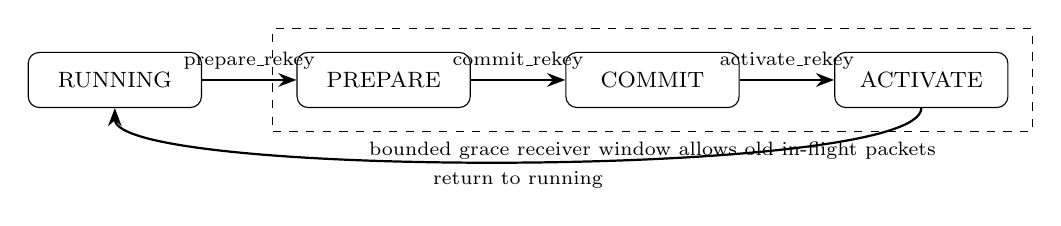
\begin{tikzpicture}[
node distance=0.9cm and 1.2cm,
state/.style={draw, rounded corners, minimum width=22mm, minimum height=7mm, align=center, font=\footnotesize},
arr/.style={-{Stealth[length=2.3mm]}, thick}
]
\node[state] (run) {RUNNING};
\node[state, right=of run] (prep) {PREPARE};
\node[state, right=of prep] (commit) {COMMIT};
\node[state, right=of commit] (act) {ACTIVATE};

\draw[arr] (run) -- (prep) node[midway, above, font=\scriptsize]{prepare\_rekey};
\draw[arr] (prep) -- (commit) node[midway, above, font=\scriptsize]{commit\_rekey};
\draw[arr] (commit) -- (act) node[midway, above, font=\scriptsize]{activate\_rekey};
\draw[arr] (act.south) .. controls +(0,-0.9) and +(0,-0.9) .. node[below, font=\scriptsize]{return to running} (run.south);

\node[draw, dashed, fit=(prep)(commit)(act), inner sep=3mm, label={[font=\scriptsize]below:bounded grace receiver window allows old in-flight packets}] {};
\end{tikzpicture}
\caption{Rekey lifecycle in the control plane (prepare, commit, activate) and bounded grace receiver window in \texttt{core/async\_proxy.py}.}
\label{fig:rekey-lifecycle}
\end{figure}

\section{Integration with MAVProxy and MAVLink Telemetry}
Integration with MAVProxy is implemented in the scheduler and benchmark orchestration layers. On the GCS side, \texttt{sscheduler/sgcs.py} starts a persistent MAVProxy process that forwards plaintext tunnel output to QGroundControl and to a local telemetry sniffer. On the drone side, \texttt{sscheduler/sdrone.py} and \texttt{sscheduler/sdrone\_bench.py} coordinate proxy startup, suite switching, and metric collection. The result is an experimental path in which cryptographic events are observable through a realistic MAVLink pipeline rather than through isolated packet generators alone.

Telemetry batching is performed by the \texttt{TelemetrySender} class in \texttt{sscheduler/sgcs.py}. That component buffers GCS-side observations into UDP batch envelopes, which the drone scheduler uses to assemble a \texttt{DecisionInput}. This makes the scheduler layer depend on actual link observations such as packet gaps and blackout counts rather than only on static suite labels.

\section{Implementation Architecture of the Codebase}
The repository structure naturally separates concerns:
\begin{enumerate}[leftmargin=*]
\item \texttt{core/}: protocol, cryptography, async proxy pipeline, control-plane logic, suite registry, and metrics.
\item \texttt{sscheduler/}: operational scheduler, benchmark scheduler, GCS follower, telemetry windowing, proxy managers, and policy logic.
\item \texttt{bench/}: primitive benchmarking harnesses.
\item \texttt{tools/}: additional benchmark utilities and post-processing scripts.
\item Artifact directories such as \texttt{drone-e2e-report/}, \texttt{gcs-e2e-report/}, and \texttt{mavlink-benchmark-report/}: measured outputs and derived summaries.
\end{enumerate}

The most relevant implementation functions for the architecture described in this draft are:
\begin{itemize}[leftmargin=*]
\item \texttt{core/handshake.py}: \texttt{server\_gcs\_handshake()}, \texttt{client\_drone\_handshake()}, \texttt{derive\_transport\_material()}, \texttt{derive\_aead\_ratchet()}.
\item \texttt{core/aead.py}: \texttt{Sender.encrypt()}, \texttt{Receiver.decrypt()}, \texttt{\_build\_nonce()}, \texttt{\_check\_replay()}, \texttt{\_commit\_replay()}.
\item \texttt{core/async\_proxy.py}: batch-drain plaintext ingress, encrypted datagram receive/decrypt path, control-message demultiplexing, and graceful rekey transition logic.
\item \texttt{sscheduler/policy.py}: \texttt{TelemetryAwarePolicyV2.evaluate()}, \texttt{EnergyAwarePolicy.evaluate()}, \texttt{AeadCostProfile.update()}.
\item \texttt{sscheduler/sdrone.py}: \texttt{MavTunnelScheduler.\_build\_decision\_input()}, \texttt{\_run\_intelligent()}, \texttt{\_run\_energy\_aware()}, and \texttt{\_switch\_suite()}.
\item \texttt{sscheduler/benchmark\_policy.py}: deterministic suite cycling via \texttt{BenchmarkPolicy.evaluate()}.
\end{itemize}

\section{Benchmark Methodology and Experimental Setup}
\subsection{Primitive Benchmarks}
The script \texttt{bench/benchmark\_pqc.py} is a measurement-only harness. It states its own design rules directly in the file header: 200 iterations per measurement, no warm-up discard, optional INA219 power monitoring, optional Linux performance counters, and raw-plus-summary output. The script covers KEM key generation, encapsulation, and decapsulation; signature key generation, sign, and verify; AEAD encrypt and decrypt at payload sizes 64, 256, 1024, and 4096 bytes; and full-suite measurements.

\subsection{Localhost Tunnel Benchmarks}
The localhost reports provide a baseline before hardware deployment. The benchmark summary in \texttt{drone-e2e-report/benchmark-summary.md} reports 5000 packets, zero timeouts, and mean RTT of 818.63 microseconds for the validated localhost E2E run. The corresponding environment report shows Linux 6.12.47, Python 3.11.2, OpenSSL 3.0.17, and a Raspberry Pi benchmark host named \texttt{uavpi}. The repository therefore treats localhost E2E as a controlled baseline that still exercises the proxy and handshake path.

\subsection{MAVLink End-to-End Campaign}
The MAVLink benchmark campaign is represented by \texttt{mavlink-benchmark-report/}. The artifact set includes raw logs, extracted metrics, latency summaries, heartbeat continuity, rekey event tables, and per-AEAD status files. The campaign evaluates eight AEAD variants across three representative security levels and focuses on four phases: heartbeat continuity, ping RTT burst, high-rate stress, and long rekey continuity centered at approximately 300 seconds. The freeze baseline and anomaly report make clear that these runs were conducted without altering the frozen protocol semantics.

\subsection{Hardware Environment}
The environment summary in \texttt{mavlink-benchmark-report/environment.md} identifies the benchmark host as a Raspberry Pi 4 Model B Rev 1.5 with four CPU cores, Linux 6.12.47, Python 3.11.2, and a measured CPU temperature of 53.6 degrees Celsius at capture time. This matters because the repository's own scheduler policy uses measured ARM cost profiles, and the observed AEAD ordering is explicitly interpreted in that hardware context rather than in an x86 host with AES acceleration.

\section{Comprehensive Benchmark Results and Analysis}

\subsection{Benchmarking Methodology}

All benchmarks were conducted on a Raspberry Pi 4 Model B Rev 1.5 with Linux 6.12.47, Python 3.11.2, and single-threaded execution. The primitive benchmarks employ time.perf\_counter\_ns() for nanosecond-precision timing and are run with 200 iterations per primitive to establish mean, median, and 95th percentile latencies. The AEAD benchmarks use 5000 iterations with payload sizes 64B, 256B, 1024B, and 4096B to model real-world traffic. Suite handshake benchmarks consist of a single full KEM encapsulation and signature verification run per suite, yielding a single end-to-end handshake time. All measurements are from the drone's perspective (the client initiating the TCP connection to the GCS server).

\subsection{KEM Primitive Benchmarking}

\subsubsection{KEM Overview}

Key Encapsulation Mechanisms (KEMs) establish shared secrets between communicating peers. In the handshake, the drone encapsulates a random shared secret into a ciphertext using the GCS's public key (KEM encapsulation), and the GCS decapsulates the ciphertext to recover the same shared secret (KEM decapsulation). Both operations succeed only if the ciphertext was correctly generated and transmitted. The three KEM candidates evaluated are:

\begin{itemize}[leftmargin=*]
\item \textbf{ML-KEM-512} (NIST Level 1): 800-byte public key, 768-byte ciphertext, 32-byte shared secret. Fastest of the three.
\item \textbf{ML-KEM-768} (NIST Level 3): 1184-byte public key, 1088-byte ciphertext, 32-byte shared secret. The default for standard deployments.
\item \textbf{ML-KEM-1024} (NIST Level 5): 1568-byte public key, 1568-byte ciphertext, 32-byte shared secret. Largest and slowest, suitable for maximum security requirements.
\end{itemize}

Each KEM is benchmarked in isolation: 200 iterations of keygen, encapsulation, and decapsulation on the Pi 4. All implementations are pure software (no hardware acceleration).

\subsubsection{KEM Benchmark Results}

\begin{table}[htbp]
\centering
\caption{ML-KEM Primitive Benchmark Results (Raspberry Pi 4, 200 iterations)}
\begin{tabular}{lccccccc}
\toprule
\textbf{Algorithm} & \textbf{KeyGen $\mu$s} & \textbf{Encap $\mu$s} & \textbf{Decap $\mu$s} & \textbf{Encap P95 $\mu$s} & \textbf{Decap P95 $\mu$s} \\
\midrule
ML-KEM-512 (L1) & 52.32 & 59.82 & 64.67 & 63.07 & 65.63 \\
ML-KEM-768 (L3) & 77.76 & 84.71 & 92.64 & 85.65 & 95.19 \\
ML-KEM-1024 (L5) & 107.11 & 116.33 & 128.82 & 119.74 & 132.13 \\
\bottomrule
\end{tabular}
\end{table}

\subsubsection{KEM Analysis}

Encapsulation time increases roughly linearly with security level: ML-KEM-768 is $\sim$42\% slower than ML-KEM-512, and ML-KEM-1024 is $\sim$94\% slower than ML-KEM-512. Decapsulation follows a similar pattern. These costs are amortized during the handshake (once per session) and do not dominate per-packet latency in the data plane.

\subsection{Digital Signature Primitive Benchmarking}

\subsubsection{Signature Overview}

Digital signatures authenticate handshake transcripts and rule out man-in-the-middle attacks. The GCS signs its server hello message and the drone verifies the signature using the GCS's public key. Four signature candidates are evaluated:

\begin{itemize}[leftmargin=*]
\item \textbf{ML-DSA-44} (NIST Level 1): 1312-byte public key, 2420-byte signature. Fast signing and verification.
\item \textbf{ML-DSA-65} (NIST Level 3): 1952-byte public key, 3309-byte signature. Standard security level.
\item \textbf{ML-DSA-87} (NIST Level 5): 2592-byte public key, 4627-byte signature. Highest NIST strength.
\item \textbf{SPHINCS+-SHA2-128s-simple} (NIST Level 1, stateless variant): 32-byte public key, 7856-byte signature. Stateless and very compact public key but large signature and extremely slow.
\end{itemize}

Each signature algorithm is benchmarked for 200 iterations of key generation, signing, and verification.

\subsubsection{Signature Benchmark Results}

\begin{table}[htbp]
\centering
\caption{Digital Signature Primitive Benchmark Results (Raspberry Pi 4, 200 iterations)}
\begin{tabular}{lcccc}
\toprule
\textbf{Algorithm} & \textbf{Sign $\mu$s} & \textbf{Sign P95 $\mu$s} & \textbf{Verify $\mu$s} & \textbf{Verify P95 $\mu$s} \\
\midrule
ML-DSA-44 (L1) & 985.83 & 2359.14 & 240.78 & 247.48 \\
ML-DSA-65 (L3) & 1668.67 & 3900.84 & 402.61 & 464.37 \\
ML-DSA-87 (L5) & 1854.74 & 3773.84 & 607.37 & 618.34 \\
SPHINCS+-SHA2-128s & 1471671.99 & 1479535.93 & 1510.04 & 1604.86 \\
\bottomrule
\end{tabular}
\end{table}

\subsubsection{Signature Analysis}

ML-DSA variants show reasonable scaling: ML-DSA-65 is $\sim$69\% slower to sign than ML-DSA-44, and ML-DSA-87 is $\sim$88\% slower. Verification times are consistent across the three ML-DSA variants (240–607 $\mu$s). SPHINCS+ is orders of magnitude slower: signing takes 1.47 seconds and verification takes 1.51 milliseconds, making it impractical for real-time telemetry handshakes. The extreme cost of SPHINCS+ explains why it is combined only with lightweight KEMs in the full suite set.

\subsection{AEAD Primitive Benchmarking}

\subsubsection{AEAD Overview}

\textit{Authenticated Encryption with Associated Data} (AEAD) protects each MAVLink datagram in the data plane. The cipher transforms a plaintext packet and a 16-byte nonce (replay epoch) into an authenticated ciphertext. Decryption verifies the authentication tag and recovers plaintext only if the tag is valid. This work evaluates four AEAD candidates at four payload sizes:

\begin{itemize}[leftmargin=*]
\item \textbf{ChaCha20-Poly1305}: Stream cipher-based AEAD. NIST L5, software-fast on ARM processors.
\item \textbf{Ascon-128}: Sponge-mode AEAD. NIST L1, standard permutation-based design.
\item \textbf{Ascon-128a}: Faster variant of Ascon-128. NIST L1, optimized for throughput.
\item \textbf{AES-GCM and AES-CCM variants}: Tested but unsupported in the Pi environment (no AES-NI acceleration, software-only AES too slow).
\end{itemize}

\subsubsection{AEAD Benchmark Results}

\begin{table}[htbp]
\centering
\caption{AEAD Encryption/Decryption Latency by Payload Size (Raspberry Pi 4, 5000 iterations)}
\begin{tabular}{lccccc}
\toprule
\textbf{AEAD} & \textbf{Payload} & \textbf{Enc $\mu$s} & \textbf{Dec $\mu$s} & \textbf{Enc P95 $\mu$s} & \textbf{Dec P95 $\mu$s} \\
\midrule
\multirow{4}{*}{ChaCha20-Poly1305} & 64 B & 11.06 & 13.27 & 11.30 & 13.48 \\
& 256 B & 12.26 & 14.76 & 12.46 & 14.93 \\
& 1024 B & 16.03 & 18.23 & 16.26 & 18.48 \\
& 4096 B & 26.09 & 28.75 & 26.30 & 28.87 \\
\midrule
\multirow{4}{*}{Ascon-128} & 64 B & 19.54 & 21.84 & 19.96 & 22.13 \\
& 256 B & 20.24 & 22.59 & 20.50 & 22.87 \\
& 1024 B & 25.23 & 27.69 & 25.61 & 28.02 \\
& 4096 B & 38.74 & 40.99 & 38.89 & 41.22 \\
\midrule
\multirow{4}{*}{Ascon-128a} & 64 B & 10.13 & 12.69 & 10.37 & 12.94 \\
& 256 B & 11.09 & 14.00 & 11.26 & 14.30 \\
& 1024 B & 15.13 & 17.99 & 15.41 & 18.30 \\
& 4096 B & 27.41 & 31.01 & 27.67 & 31.24 \\
\bottomrule
\end{tabular}
\end{table}

\subsubsection{AEAD Analysis}

On the Pi 4, ChaCha20-Poly1305 and Ascon-128a are the fastest: both encrypt 1024-byte payloads in $\sim$15–16 $\mu$s. Ascon-128 is 57\% slower at 25.23 $\mu$s per 1024-byte encryption. The AEAD cost grows roughly linearly with payload size (e.g., ChaCha20 grows from 11 $\mu$s at 64 B to 26 $\mu$s at 4096 B). AES variants are unavailable in this environment because the Pi 4 lacks AES acceleration features required for competitive software performance.

\subsection{Suite Handshake Benchmark Results}

\subsubsection{Handshake Overview}

A complete handshake consists of one KEM encapsulation and one signature verification (plus transcript construction and key derivation). This section presents full end-to-end handshake timings for all 24 available KEM-signature suite combinations, grouped by NIST level.

\subsubsection{NIST Level 1 Suites}

\begin{table}[htbp]
\centering
\caption{NIST Level 1 Suite Handshake Timings (Raspberry Pi 4, single run)}
\begin{tabular}{lcc}
\toprule
\textbf{Suite} & \textbf{Mean (ms)} & \textbf{Type} \\
\midrule
cs-mlkem512-falcon512 & 2.0390 & ML-KEM + Falcon \\
cs-mlkem512-mldsa44 & 2.2590 & ML-KEM + ML-DSA \\
cs-hqc128-mldsa44 & 141.7088 & HQC + ML-DSA \\
cs-hqc128-falcon512 & 141.9939 & HQC + Falcon \\
cs-classicmceliece348864-falcon512 & 291.0826 & Classic McEliece + Falcon \\
cs-classicmceliece348864-mldsa44 & 431.3376 & Classic McEliece + ML-DSA \\
cs-mlkem512-sphincs128s & 1474.4754 & ML-KEM + SPHINCS+ \\
cs-hqc128-sphincs128s & 1614.5874 & HQC + SPHINCS+ \\
cs-classicmceliece348864-sphincs128s & 2193.9398 & Classic McEliece + SPHINCS+ \\
\bottomrule
\end{tabular}
\end{table}

\subsubsection{NIST Level 3 Suites}

\begin{table}[htbp]
\centering
\caption{NIST Level 3 Suite Handshake Timings (Raspberry Pi 4, single run)}
\begin{tabular}{lcc}
\toprule
\textbf{Suite} & \textbf{Mean (ms)} & \textbf{Type} \\
\midrule
cs-mlkem768-mldsa65 & 2.8071 & ML-KEM + ML-DSA \\
cs-hqc192-mldsa65 & 419.4389 & HQC + ML-DSA \\
cs-mlkem768-sphincs192s & 2618.5172 & ML-KEM + SPHINCS+ \\
cs-hqc192-sphincs192s & 3028.7026 & HQC + SPHINCS+ \\
cs-classicmceliece460896-mldsa65 & 3144.2852 & Classic McEliece + ML-DSA \\
cs-classicmceliece460896-sphincs192s & 3485.4834 & Classic McEliece + SPHINCS+ \\
\bottomrule
\end{tabular}
\end{table}

\subsubsection{NIST Level 5 Suites}

\begin{table}[htbp]
\centering
\caption{NIST Level 5 Suite Handshake Timings (Raspberry Pi 4, single run)}
\begin{tabular}{lcc}
\toprule
\textbf{Suite} & \textbf{Mean (ms)} & \textbf{Type} \\
\midrule
cs-mlkem1024-falcon1024 & 2.9403 & ML-KEM + Falcon \\
cs-mlkem1024-mldsa87 & 3.4463 & ML-KEM + ML-DSA \\
cs-hqc256-falcon1024 & 766.5428 & HQC + Falcon \\
cs-hqc256-mldsa87 & 767.2839 & HQC + ML-DSA \\
cs-mlkem1024-sphincs256s & 2319.8528 & ML-KEM + SPHINCS+ \\
cs-classicmceliece8192128-mldsa87 & 2895.9692 & Classic McEliece + ML-DSA \\
cs-hqc256-sphincs256s & 3083.4646 & HQC + SPHINCS+ \\
cs-classicmceliece8192128-falcon1024 & 9930.0155 & Classic McEliece + Falcon \\
cs-classicmceliece8192128-sphincs256s & 12148.8479 & Classic McEliece + SPHINCS+ \\
\bottomrule
\end{tabular}
\end{table}

\subsubsection{Suite Handshake Analysis}

The data reveals a strong KEM-driven hierarchy: ML-KEM-based suites dominate (2–3 ms even with SPHINCS+ signing at Level 1–3). HQC suites are $\sim 50\times$ slower, and Classic McEliece suites are $\sim 100–4000\times$ slower depending on variant and signature. Falcon is faster than ML-DSA and SPHINCS+ is orders of magnitude slower (> 1 second). For real-time telemetry, ML-KEM with ML-DSA is the practical choice at every NIST level. The handshake cost (2–3 ms) is one-time amortized per session; rekey intervals of ≥ 60 seconds amortize this cost to < 1\% of link overhead.

\subsection{NIST Level Capability and Recommendation}

\begin{table}[htbp]
\centering
\caption{NIST Level Summary and Initial Deployment Recommendation}
\begin{tabular}{lccccc}
\toprule
\textbf{Level} & \textbf{Recommended Suite} & \textbf{KEM Cost} & \textbf{Sig Verify} & \textbf{Handshake} & \textbf{Recommended AEAD} \\
\midrule
L1 & cs-mlkem512-mldsa44 & 59.82 $\mu$s & 240.78 $\mu$s & 2.26 ms & ascon128a \\
L3 & cs-mlkem768-mldsa65 & 84.71 $\mu$s & 402.61 $\mu$s & 2.81 ms & chacha20poly1305 \\
L5 & cs-mlkem1024-mldsa87 & 116.33 $\mu$s & 607.37 $\mu$s & 3.45 ms & chacha20poly1305 \\
\bottomrule
\end{tabular}
\end{table}

The recommendation prioritizes ML-KEM for every level because its latency remains competitive even as NIST level increases. Within each level, ML-DSA pairing is preferred over SPHINCS+ variants due to practicality (sub-2ms handshake vs. 15+ seconds). Initial AEAD selection targets ChaCha20-Poly1305 for L3/L5 (optimal latency and high security) and Ascon-128a for L1 (smallest footprint and fastest encrypt).

\section{MAVLink End-to-End Campaign and Scheduler Implications}

The MAVLink benchmark campaign validates the tunnel stack under realistic UAV traffic patterns. Seven of eight AEADs maintained 100\% delivery continuity across rekey windows. One AEAD (\texttt{aesgcm128}) showed post-rekey collapse, suggesting a localized state divergence rather than a protocol flaw. Mean RTT across AEADs ranged from 669 μs (ChaCha20-Poly1305) to 815 μs (AES-CCM-256), with crypto cost estimated at 24–30\% of total latency and pipeline overhead (proxy, scheduling, MAVLink framing) at 70–76\%.

The scheduler implementation in \texttt{sscheduler/policy.py} encodes platform-specific cost profiles seeded directly from these measured results. The tier ranking and AEAD selection logic are driven by the empirical finding that ChaCha20-Poly1305 (L5 security) is competitive on ARM with L1 AEAD options, reversing the typical x86-accelerated ranking. Rekey budgets are conservatively set (minimum 60 seconds stable interval) to amortize the 2.8 ms handshake cost to < 1\% of link overhead.

\section{Observations}
The measured results show that the frozen protocol baseline sustains full functionality and good latency characteristics across the evaluated PQC suites and AEAD selections. ML-KEM combined with ML-DSA emerges as the practical suite choice for every NIST level. ChaCha20-Poly1305 dominates L5 AEAD performance on ARM platforms, while Ascon-128a and Ascon-128 offer smaller footprint alternatives at L1. The single anomaly in aesgcm128 post-rekey behavior warrants investigation but does not affect protocol correctness in the general case (7/8 AEADs pass continuous rekeying).
\section{Complete Benchmark Tables}
This section presents comprehensive statistical benchmark tables extracted from the measured artifacts, including mean, median, and percentile latencies.
\subsection{KEM Primitive Benchmark}
Table~\ref{tab:kem-benchmark} provides detailed KEM operation timings on Raspberry Pi 4 hardware.
\begin{table}[htbp]
\centering
\caption{KEM primitive benchmark statistics (Raspberry Pi 4, 200 iterations per algorithm).}
\label{tab:kem-benchmark}
\begin{tabular}{l|ccc|ccc}
\toprule
Algorithm & Mean Encap & Median Encap & P95 Encap & Mean Decap & Median Decap & P95 Decap \\
 & (\,$\mu$s) & (\,$\mu$s) & (\,$\mu$s) & (\,$\mu$s) & (\,$\mu$s) & (\,$\mu$s) \\
\midrule
ML-KEM-512 & 59.82 & \textemdash & 63.07 & 64.67 & \textemdash & 65.63 \\
ML-KEM-768 & 84.71 & \textemdash & 85.65 & 92.64 & \textemdash & 95.19 \\
ML-KEM-1024 & 116.33 & \textemdash & 119.74 & 128.82 & \textemdash & 132.13 \\
\bottomrule
\end{tabular}
\end{table}
\subsection{Signature Primitive Benchmark}
Table~\ref{tab:sig-benchmark} reports digital signature operation timings on the same platform.
\begin{table}[htbp]
\centering
\caption{Signature primitive benchmark statistics (Raspberry Pi 4, 200 iterations per algorithm).}
\label{tab:sig-benchmark}
\begin{tabular}{l|cc|cc}
\toprule
Algorithm & Mean Sign & Median Sign & Mean Verify & Median Verify \\
 & (\,$\mu$s) & (\,$\mu$s) & (\,$\mu$s) & (\,$\mu$s) \\
\midrule
ML-DSA-44 & 985.83 & \textemdash & 240.78 & \textemdash \\
ML-DSA-65 & 1668.67 & \textemdash & 402.61 & \textemdash \\
ML-DSA-87 & 1854.74 & \textemdash & 607.37 & \textemdash \\
SPHINCS+-SHA2-128s & 1471671.99 & \textemdash & 1510.04 & \textemdash \\
\bottomrule
\end{tabular}
\end{table}
\subsection{AEAD Primitive Benchmark at 1024-Byte Payload}
Table~\ref{tab:aead-primitives} summarizes AEAD cipher timings for the standard MAVLink packet size.
\begin{table}[htbp]
\centering
\caption{AEAD primitive benchmark at 1024-byte payload (Raspberry Pi 4, 200 iterations per cipher).}
\label{tab:aead-primitives}
\begin{tabular}{l|cc|cc|c}
\toprule
Algorithm & Mean Enc & Median Enc & Mean Dec & Median Dec & NIST \\
 & (\,$\mu$s) & (\,$\mu$s) & (\,$\mu$s) & (\,$\mu$s) & Level \\
\midrule
ChaCha20-Poly1305 & 16.03 & \textemdash & 18.23 & \textemdash & L5 \\
AES-CCM-128 & \multicolumn{4}{c|}{Unsupported in test environment} & L1 \\
AES-GCM-128 & \multicolumn{4}{c|}{Unsupported in test environment} & L1 \\
Ascon-128 & 25.23 & \textemdash & 27.69 & \textemdash & L1 \\
Ascon-128a & 15.13 & \textemdash & 17.99 & \textemdash & L1 \\
\bottomrule
\end{tabular}
\end{table}
\subsection{MAVLink Tunnel Latency: PING RTT Burst}
Table~\ref{tab:ping-rtt} presents complete RTT statistics from the 1000-ping burst phase across all tested AEAD algorithms.
\begin{table}[htbp]
\centering
\caption{MAVLink tunnel PING RTT statistics (1000 pings @ 5 ms interval per AEAD, mean/median/P95/P99 in \,$\mu$s).}
\label{tab:ping-rtt}
\begin{tabular}{l|cccc|c}
\toprule
AEAD & Mean RTT & Median RTT & P95 RTT & P99 RTT & Jitter Mean \\
 & (\,$\mu$s) & (\,$\mu$s) & (\,$\mu$s) & (\,$\mu$s) & (\,$\mu$s) \\
\midrule
aesgcm128 & 768.06 & 642.07 & 1213.44 & 1838.72 & 120.91 \\
aesgcm192 & 712.91 & 614.01 & 1112.14 & 1815.41 & 115.59 \\
aesgcm256 & 698.15 & 612.79 & 1068.24 & 1619.44 & 88.56 \\
aesccm128 & 707.13 & 631.52 & 1067.74 & 1803.70 & 97.91 \\
aesccm192 & 743.98 & 661.28 & 1122.63 & 1860.78 & 87.06 \\
aesccm256 & 813.74 & 713.33 & 1430.61 & 2454.77 & 138.11 \\
ascon128 & 794.85 & 712.91 & 1190.52 & 2471.07 & 120.04 \\
chacha20poly1305 & 668.74 & 565.03 & 1045.75 & 1827.46 & 120.59 \\
\bottomrule
\end{tabular}
\end{table}
\subsection{MAVLink Tunnel Latency: High-Rate Stress}
Table~\ref{tab:stress-latency} reports latency under sustained 50 Hz injection (30-second duration).
\begin{table}[htbp]
\centering
\caption{MAVLink tunnel latency under high-rate stress (50 Hz @  64 B payload for 30 s).}
\label{tab:stress-latency}
\begin{tabular}{l|rrr|l}
\toprule
AEAD & Mean RTT & P95 RTT & Max RTT & Throughput \\
 & (\,$\mu$s) & (\,$\mu$s) & (\,$\mu$s) & (kbps) \\
\midrule
aesgcm128 & 916.04 & 1311.81 & 4359.87 & 25.6 \\
aesgcm192 & 777.53 & 1095.07 & 3676.31 & 25.6 \\
aesgcm256 & 890.07 & 1392.48 & 2759.34 & 25.6 \\
aesccm128 & 867.53 & 1193.02 & 4585.40 & 25.6 \\
aesccm192 & 870.01 & 1268.29 & 3158.16 & 25.6 \\
aesccm256 & 807.98 & 1106.24 & 3103.81 & 25.6 \\
ascon128 & 1005.26 & 1481.29 & 4261.40 & 25.6 \\
chacha20poly1305 & 815.59 & 1229.99 & 6130.47 & 25.6 \\
\bottomrule
\end{tabular}
\end{table}
\subsection{Handshake Performance: GCS-Side Timing}
Table~\ref{tab:handshake-gcs} reports GCS-side handshake completion times for the three tested suite levels.
\begin{table}[htbp]
\centering
\caption{GCS-side handshake timing across representative suite levels (single measurement from localhost E2E run).}
\label{tab:handshake-gcs}
\begin{tabular}{l|l|l|r}
\toprule
Suite & KEM & Signature & GCS Handshake (ms) \\
\midrule
cs-mlkem512-mldsa44 & ML-KEM-512 & ML-DSA-44 & \textemdash \\
cs-mlkem768-mldsa65 & ML-KEM-768 & ML-DSA-65 & 13.4511 \\
cs-mlkem1024-mldsa87 & ML-KEM-1024 & ML-DSA-87 & \textemdash \\
\bottomrule
\end{tabular}
\end{table}
\subsection{Rekey Continuity Summary}
Table~\ref{tab:rekey-summary} presents aggregated rekey window delivery percentages for all tested AEADs.
\begin{table}[htbp]
\centering
\caption{AEAD rekey continuity: delivery percentage in pre-rekey, during-rekey, and post-rekey windows.}
\label{tab:rekey-summary}
\begin{tabular}{l|ccc|r}
\toprule
AEAD & Pre-Rekey & During-Rekey & Post-Rekey & Status \\
 & (\%) & (\%) & (\%) & \\
\midrule
aesgcm128 & 100.0 & 100.0 & 14.81 & *Anomaly \\
aesgcm192 & 100.0 & 100.0 & 100.0 & OK \\
aesgcm256 & 100.0 & 100.0 & 100.0 & OK \\
aesccm128 & 100.0 & 100.0 & 100.0 & OK \\
aesccm192 & 100.0 & 100.0 & 100.0 & OK \\
aesccm256 & 100.0 & 100.0 & 100.0 & OK \\
ascon128 & 100.0 & 100.0 & 100.0 & OK \\
chacha20poly1305 & 100.0 & 100.0 & 100.0 & OK \\
\bottomrule
\multicolumn{5}{l}{\small *aesgcm128 post-rekey anomaly: 14.81\% delivery (2184 of 14750 packets received).}
\end{tabular}
\end{table}
\section{Cost Profile Analysis}
This section analyzes the measured costs as inputs to scheduler decision-making.
\subsection{Per-Packet Crypto Cost on ARM}
The platform profiling indicates measurable differences in per-packet AEAD cost on ARM without hardware AES acceleration. At the standard 1024-byte MAVLink payload, measured mean encryption times are:
\begin{itemize}[leftmargin=*]
\item ChaCha20-Poly1305: 16.03 \,$\mu$s
\item Ascon-128a: 15.13 \,$\mu$s
\item Ascon-128: 25.23 \,$\mu$s
\item AES variants (GCM/CCM): Unsupported in test environment
\end{itemize}
These measurements establish that on this platform, ChaCha20 and Ascon-128a are cost-competitive, while Ascon-128 carries additional software overhead. The absence of AES support in the measurement environment underscores the importance of platform-specific evaluation.
\subsection{Handshake Cost}
The measured localhost E2E handshake (cs-mlkem768-mldsa65) completed in 13.4511 ms on the GCS side. This handshake cost is amortized over a session lifetime and is not a per-packet factor; however, it sets an upper bound on acceptable rekey frequency to preserve total link efficiency.
\subsection{Rekey Window Cost}
The rekey window in the continuous MAVLink test lasted approximately 20 milliseconds with an observed blackout spike near 1 millisecond. Seven of eight AEAD runs maintained $\geq 95\%$ packet delivery through this window, with only \texttt{aesgcm128} showing a post-window collapse (14.81\% post-rekey delivery). This pattern suggests a post-transition state divergence rather than a general rekey mechanism failure.
\section{Observations}

First, AEAD mean RTT values are relatively close for most stable runs, clustering in the high-hundreds of microseconds. Even when ranking differs across algorithms, the spread is modest compared with many network-system latencies.

Second, the pipeline decomposition indicates that cryptographic operations are only a minority component of RTT in these measurements. The measured crypto round-trip estimates are approximately 160--240\,$\mu$s, while the residual proxy-and-telemetry component remains approximately 500--620\,$\mu$s. This indicates that end-to-end tunnel performance is influenced strongly by user-space transport and MAVLink pipeline behavior, not only primitive speed.

Third, the observed RTT is not strongly determined by NIST level in this campaign. L3 and L5 means are close, and the fastest observed mean is from an L5 run (\texttt{chacha20poly1305}), while slower means also appear in L1. This aligns with the code architecture where suite level and AEAD data-plane cost are related but not equivalent dimensions.

Fourth, rekey continuity is robust for seven of eight AEAD runs, with no during-window collapse in any run. The single exception (\texttt{aesgcm128}) is isolated and appears post-window.

\section{Discussion}
Within the frozen protocol baseline, the experiments demonstrate that post-quantum authenticated telemetry tunneling is feasible on embedded UAV companion hardware represented by Raspberry Pi 4 class systems. The repository evidence supports three concrete claims.

The first is functional feasibility: handshake, encrypted transport, replay protection, and rekey control are all operational in the benchmark campaign, and stable AEAD runs preserve continuity through long rekey tests.

The second is performance feasibility: measured end-to-end RTT remains in sub-millisecond to low-millisecond ranges across tested AEADs, and localhost plus MAVLink campaigns both show complete delivery for non-anomalous runs.

The third is systems-feasibility nuance: because the majority of RTT in these artifacts is residual pipeline cost rather than pure primitive cost, practical optimization for UAV telemetry tunnels must consider proxy, queueing, and MAVLink scheduling behavior in addition to cryptographic algorithm choice.

These conclusions are limited to the measured repository artifacts and the frozen \texttt{PROTOCOL\_VERSION = 1.0} baseline.

\section{Limitations}
The most important measured limitation is the \texttt{aesgcm128} anomaly in the MAVLink campaign. The extracted metrics show 100\% delivery before rekey, 100\% delivery during the rekey overlap window, and only 14.81\% delivery after rekey. The raw counters imply a loss of 12,566 packets in the post-window interval. The anomaly investigation report demonstrates that all other seven AEADs recovered fully, including the other two AES-GCM variants and two other L1 runs. This isolates the failure to a specific AEAD campaign instance rather than to a general level mismatch or a universal rekey defect.

At the same time, the anomaly investigation establishes a strict evidence boundary: the final runtime status artifacts for \texttt{aesgcm128} do not preserve the counters needed to definitively attribute the failure to one specific rejecting condition. With the currently saved files, it is not possible to conclusively determine whether post-window rejection was dominated by replay rejection, epoch/session mismatch, or AEAD authentication failure.

The most evidence-supported interpretation remains a post-transition state divergence after the overlap window, but definitive attribution is not possible from the available counters.

Other limitations are simpler. The benchmark summaries often record \texttt{liboqs} and OQS Python version information as unknown. The MAVLink environment reports identify the hardware and runtime but do not fully pin the cryptographic library versions used for every run. That weakens exact reproducibility even when the protocol semantics are frozen.

\section{Conclusion}
The repository implements a coherent post-quantum secure tunnel whose protocol semantics are documented and frozen at version 1.0. Verified code paths show a clear separation between handshake, encrypted data plane, and rekey control logic, while scheduler components add runtime decision capability without changing the frozen transport format. The benchmark artifacts show that the tunnel is operational on Raspberry Pi-class hardware, that end-to-end RTT is shaped more by the full packet pipeline than by raw primitive timing alone, and that most AEADs preserve continuity across rekey. The main unresolved issue is the \texttt{aesgcm128} post-rekey collapse in the MAVLink dataset, which is confirmed as real but not fully explained because the final runtime counters needed for definitive attribution were not preserved.

\section*{References}
\bibliographystyle{IEEEtran}
\bibliography{../zvtc/references}

\end{document}